\section{Data models}

% Say something about how the graph is implemented and a reference to the book.
\subsection{DPF metamodeling}
\subsection{Entity model}

We will now present the entity model by showing en excerpt, hiding away the details. This will let us easier focus on the concepts and the flow, as the model itself is quite large and complex. See figure \ref{fig:EntityGraphExcerpt}

The entity graph shows a specific patient at a certain point or time in the clinical encounter. The patient comes to the emergency clinic. He has some symptoms which the clinician needs to uncover, by doing examinations and asking questions about the patients conditions. What the patient or caregiver tells is modelled as history, while quick examinations such as listening to the chest, looking at the skin, count the number of breaths per minute are modelled in the examination vertex. In some cases the clinician wants to test which require more time and resources, such as MRI scan, spirometry or blood tests, which are modelled as investigations.

Based on the the symptoms collected in history, examination and investigation, the clinician will set a diagnosis. The procedures for what to do with a patient with a given diagnosis is modelled under management. Hospitalization is to change the patients status to outpatient, or inpatient if he is admitted into the hospital. He might need some medication or be given advise for how he should deal with his condition the in every day life. Here the model can be expanded with routines found in other guidelines, we have identified surgery as an example. 
\begin{figure}[h!]
	\caption {An excerpt of the entity graph. Entity graph represents a patient at a certain point in the clinical encounter}
	\label{fig:EntityGraphExcerpt}
	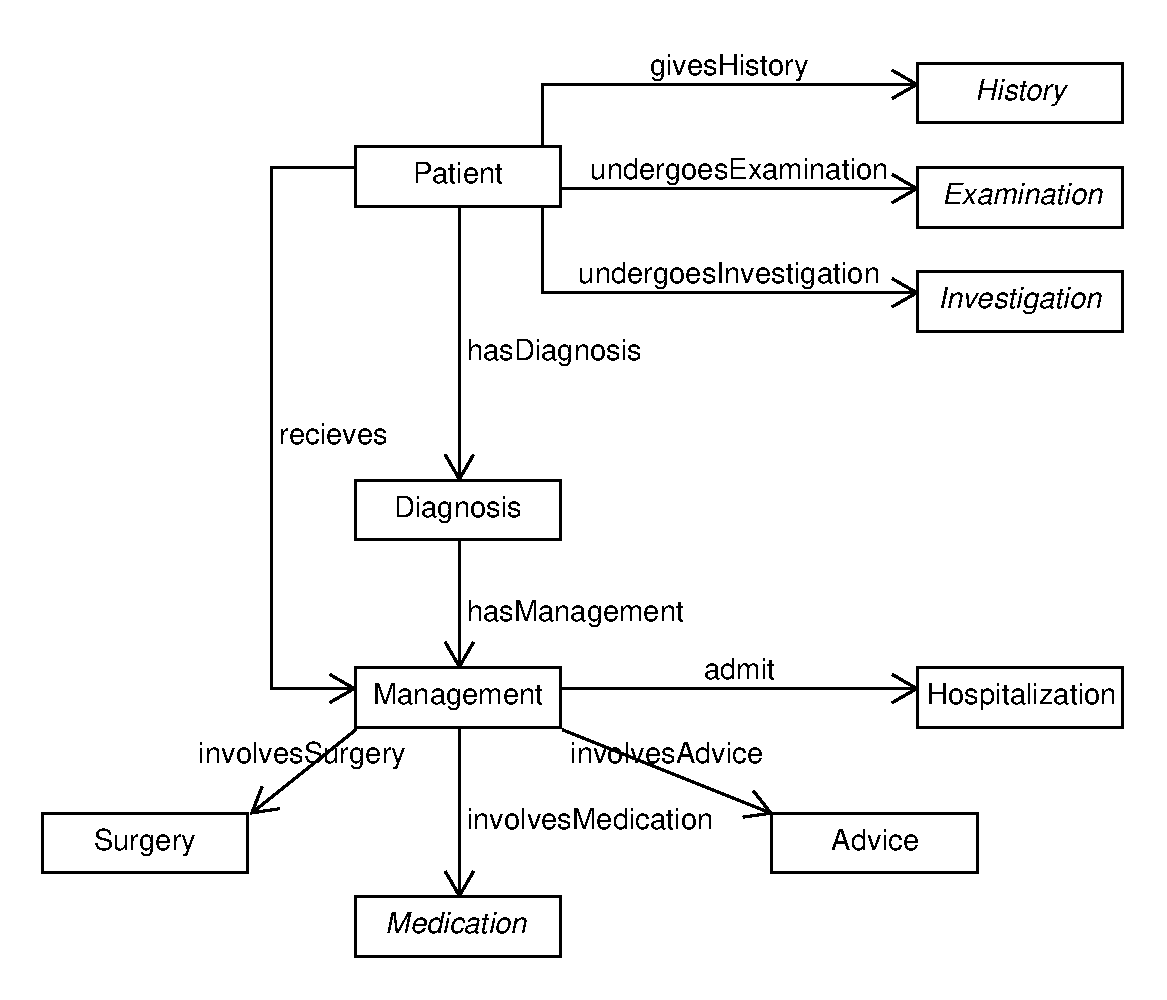
\includegraphics[scale=0.6]{EntityGraphExcerpt}
\end{figure}

In figure \ref{fig:EntityGraphPatientDiagnosis} we have expanded the Patient and Diagnosis vertices to reveal more details. PatientName and Gender, identifies the patient with a name and gender. These attributes are important when presenting a patient and his condition in a narrative or scenario. By using a name, it is easier for the reader to see that this is the same patient in different stages of the clinical encounter.

A diagnosis has a name. In the paediatric possible asthma guideline \cite{RepublicofKeny2016}, the diagnosis has a severity. A lot of medical conditions doesn't have a severity, or they are classified in another way. Here the model needs to be expanded to support other CPGs. 
\begin{figure}[h!]
	\caption {Showing the details of the Patient and Diagnosis vertices of the entity graph}
	\label{fig:EntityGraphPatientDiagnosis}
	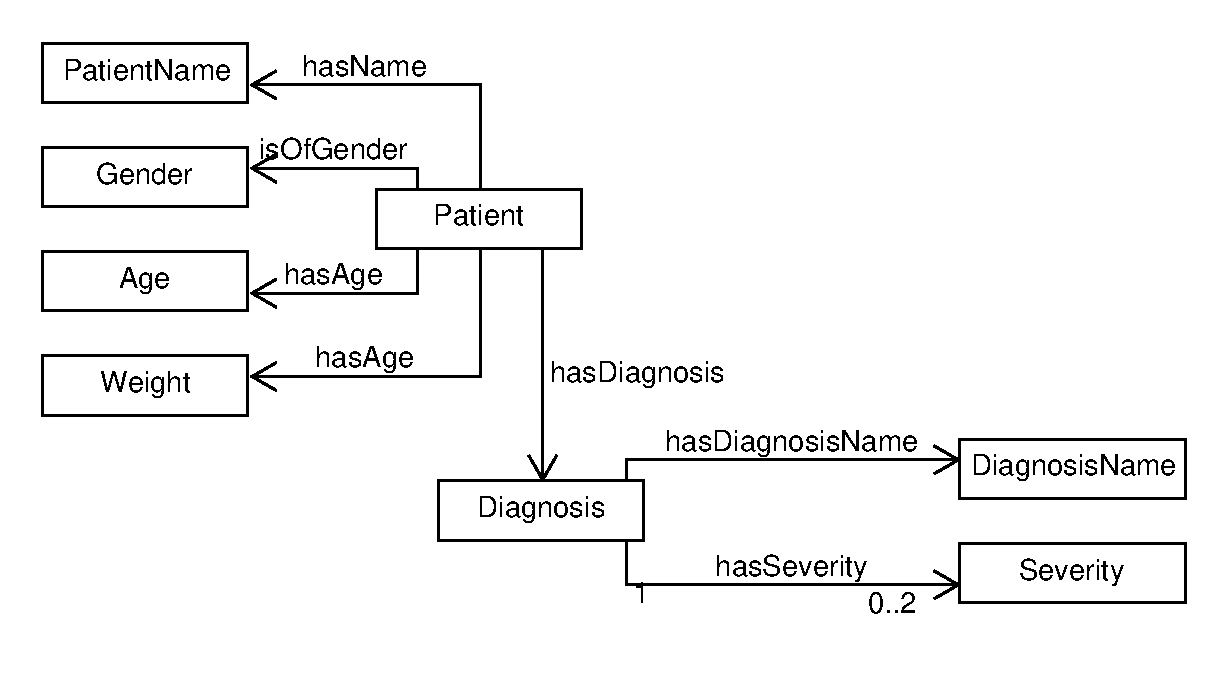
\includegraphics[scale=0.6]{EntityGraphPatientDiagnosis}
\end{figure}

In figure \ref{fig:EntityGraphHistory} we have shown our implementation of the History vertex from figure \ref{fig:EntityGraphExcerpt}. History is what the patient or the caregiver tells about the patient's condition. In the paediatric possible asthma guideline \cite{RepublicofKeny2016} we have identified three symptoms which the clinician can ask the patient or the caregiver about. Here we introduce inheritance, where the specific symptoms inherits the examination vertex. Each symptom the patient or caregiver tell about, will have a measurement. In this specific case, all the history symptoms are boolean. Either they have the symptom or they don't. The symptom values inherits from a Measurement vertex.

\begin{figure}[h!]
	\caption {Showing the implementation of History in the entity graph. What the patient or caregiver tell about the patient's condition}
	\label{fig:EntityGraphHistory}
	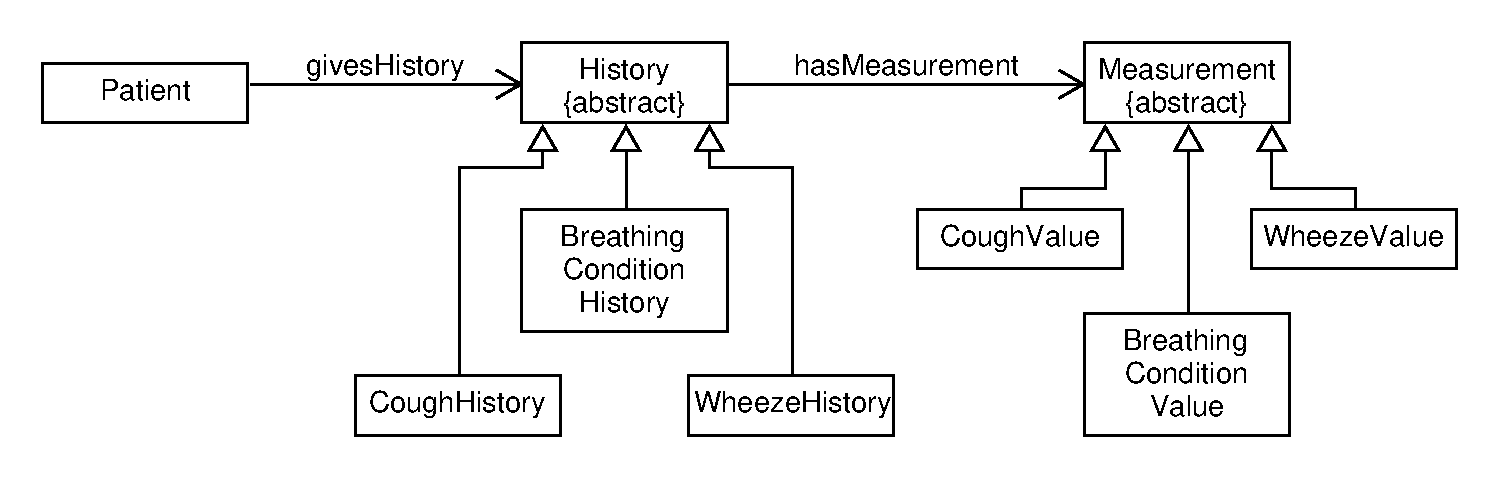
\includegraphics[scale=0.6]{EntityGraphHistory}
\end{figure}

For Examination we follow the same principles as History. We implement it by letting each symptom inherit an Examination vertex. Each symptom has value which inherits from a Measurement vertex. In figure \ref{fig:EntityGraphExamination} we have shown the inheritances with one arrow and a box. This is of practical reasons when drawing, as there are so many symptoms and it will be confusing to draw an arrow for each of them. Here the values which are stored are a bit more mixed than for History. Consciousness is measured using an AVPU scale, where A is the patient is Alert, V is Verbal, P is responding to pain and U unconscious. These are enumerates, where we store either A, V, P or U. Pulse Rate, Respiratory Rate, Oxygen Saturation are all numerical values. The other symptoms are registered as boolean values.
\textcolor{red}{Should I mention clan morphism? I am not sure I have implemented it as it is defined in the papers}
\textcolor{red}{There is a possibility that a patient tells about a symptom and when the clinician examines the symptom, he finds something else. I haven't asked Job about this, and I don't think it matters for our game.}

The implementation of Investigation would be just as we did with History and Examination. For asthma they use a lab test called spirometry, but it is not included in the paediatric possible asthma guideline \cite{RepublicofKeny2016}, so we don't include it in our model

\begin{figure}[h!]
	\caption {Showing the implementation of History in the entity graph. What the patient or caregiver tell about the patient's condition}
	\label{fig:EntityGraphExamination}
	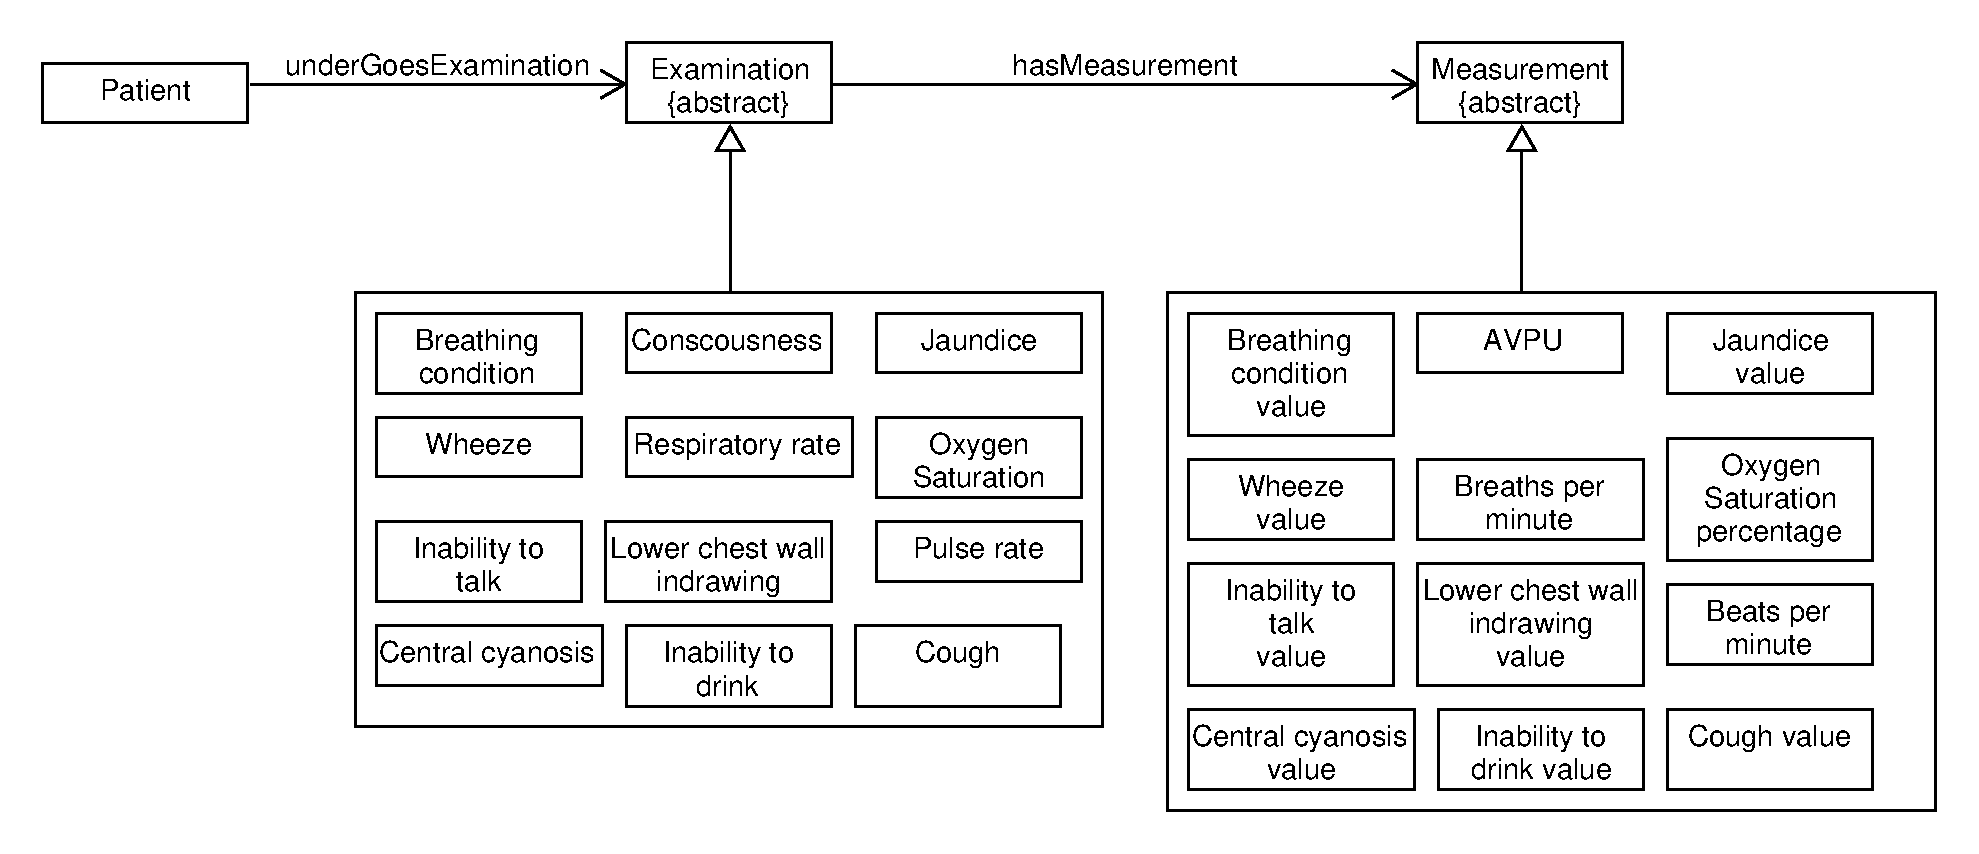
\includegraphics[scale=0.45]{EntityGraphExamination}
\end{figure}

In the paediatric possible asthma guideline \cite{RepublicofKeny2016}, there are used six medications to treat the patient. I will talk about each medicine in the model, as they are being administered differentially. Medication is modelled in figure \ref{fig:EntityGraphMedication}.


\begin{itemize}
	\item \textbf{Oxygen} is a medication. The CPG doesn't think it is necessary to elaborate on how giving it to the patient.
	
	\item For \textbf{antibiotics}, the CPG refers to a separate guideline just for administering antibiotics and is therefore out of this scope. For this reason, we just say administer antibiotics here, and don't go into the details.
	
	\item \textbf{Prednisolone} is a steroid. The clinician will administer a low dosage and increase the dosage over time until getting the desired effect. The clinician will then decrease the dosage over time to stop the treatment. For this reason we have a dosage vertex in the model, which represents the current dosage of prednisolone administered to the patient. The dosage will change as the clinician adjust it. Prednisolone has a duration vertex, as the medication should be administered for 3-5 days.
	
	\item \textbf{Corticosteroid} is another steroid, which is given to in scenarios of recurrence asthma symptoms. The CPG specifies that corticosteroid should be inhaled. This is represented in the model by the Route vertex, where other medication can be inhaled, injected, taken orally (as with pills) as some examples. The method the which will be used to inhale corticosteroid is represented by the Form-vertex. The Form is MDI with spacer, preferably with spacer with face mask. Form and Route are represented by strings as free text. However, we could make predefined vertices which inherits Corticosteroid-Route to give the content author to choose from. The Route of a medication is quite limited compared to Form for all medications.
	
	\item \textbf{Salbutamol} is inhaled to open the airways of an asthma patient. It is modelled much like corticosteroid, except it has a Rate vertex. The Rate vertex tells at which rate the patient should be taking salbutamol. Asthma patient is given salbutamol at a rate of 2.5mg per hour. The Duration is up to one hour or three doses if needed.
	
	\item \textbf{Ipratropium bromide} is modelled much like salbutamol with a Rate and a Duration. The CPG doesn't specify a route or a method.
\end{itemize}

 
 \textcolor{red}{Talk to Job about this model tomorrow. Oxygen, prednisolone and ipratopium bromide may all have a route and form. Talk to Job also about evaluation.}
\begin{figure}[h!]
	\caption {Showing the implementation of History in the entity graph. What the patient or caregiver tell about the patient's condition}
	\label{fig:EntityGraphMedication}
	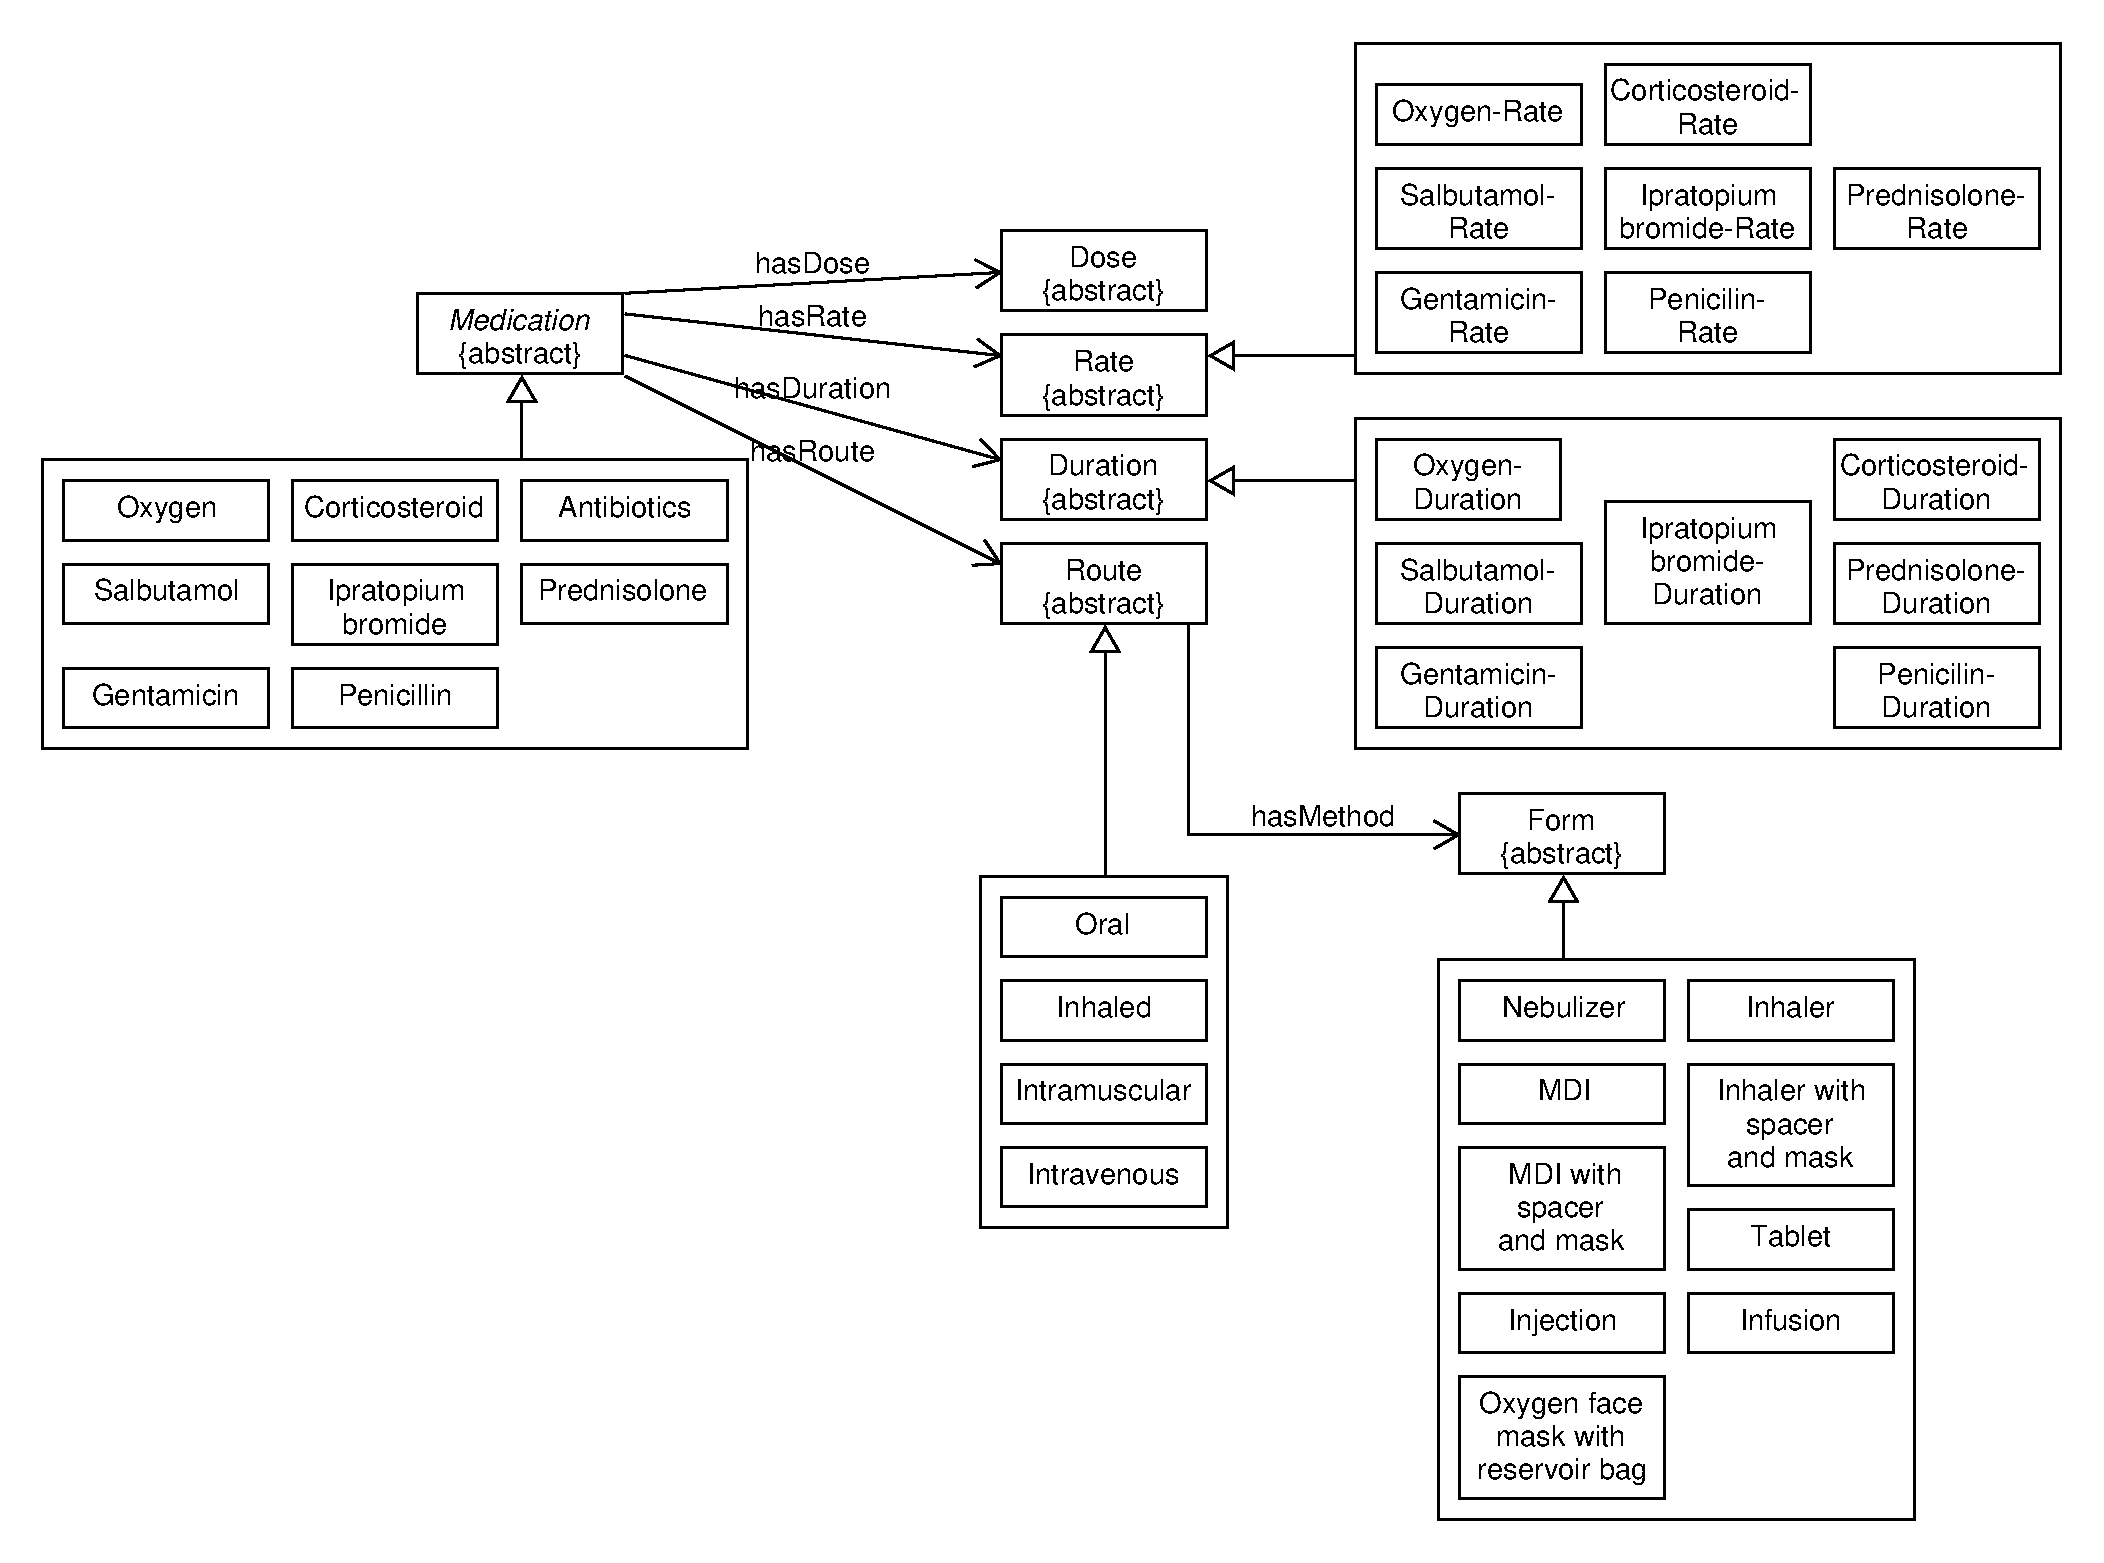
\includegraphics[scale=0.45]{EntityGraphMedication}
\end{figure}





\subsection{Workflow model}
\begin{figure}[h!]
	\caption {The workflow models is a model of the clinical encounter}
	\label{fig:WorkflowGraph}
	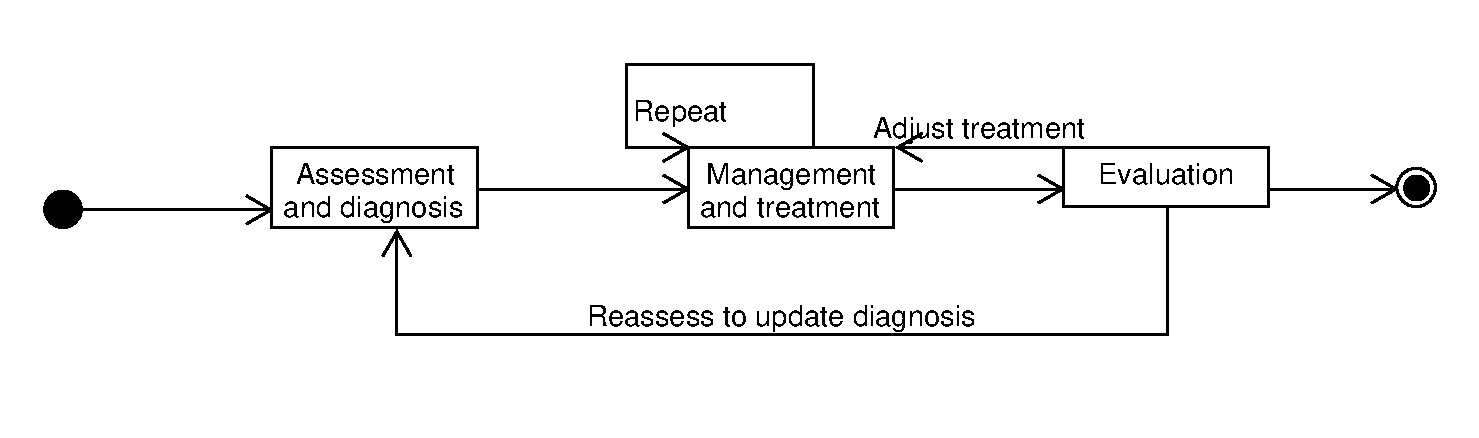
\includegraphics[scale=0.6]{WorkflowGraph}
\end{figure}


\subsection{Game model}